\chapter{Graph search}

This chapter introduces two fundamental
graph algorithms:
depth-first search and breadth-first search.
Both algorithms are given a starting
node in the graph,
and they visit all nodes that can be reached
from the starting node.
The difference in the algorithms is the order
in which they visit the nodes.

\section{Depth-first search}

\index{depth-first search}

\key{Depth-first search} (DFS)
is a straightforward graph search technique.
The algorithm begins at a starting node,
and proceeds to all other nodes that are
reachable from the starting node using
the edges in the graph.

Depth-first search always follows a single
path in the graph as long as it finds
new nodes.
After this, it returns back to previous
nodes and begins to explore other parts of the graph.
The algorithm keeps track of visited nodes,
so that it processes each node only once.

\subsubsection*{Example}

Let's consider how depth-first search processes
the following graph:
\begin{center}
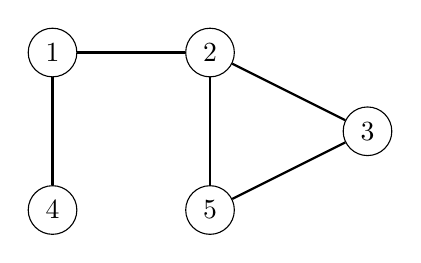
\begin{tikzpicture}
\node[draw, circle] (1) at (1,5) {$1$};
\node[draw, circle] (2) at (3,5) {$2$};
\node[draw, circle] (3) at (5,4) {$3$};
\node[draw, circle] (4) at (1,3) {$4$};
\node[draw, circle] (5) at (3,3) {$5$};

\path[draw,thick,-] (1) -- (2);
\path[draw,thick,-] (2) -- (3);
\path[draw,thick,-] (1) -- (4);
\path[draw,thick,-] (3) -- (5);
\path[draw,thick,-] (2) -- (5);
\end{tikzpicture}
\end{center}
The algorithm can begin at any node in the graph,
but we will now assume that it begins
at node 1.

The search first proceeds to node 2:
\begin{center}
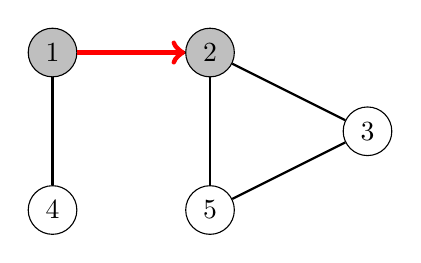
\begin{tikzpicture}
\node[draw, circle,fill=lightgray] (1) at (1,5) {$1$};
\node[draw, circle,fill=lightgray] (2) at (3,5) {$2$};
\node[draw, circle] (3) at (5,4) {$3$};
\node[draw, circle] (4) at (1,3) {$4$};
\node[draw, circle] (5) at (3,3) {$5$};

\path[draw,thick,-] (1) -- (2);
\path[draw,thick,-] (2) -- (3);
\path[draw,thick,-] (1) -- (4);
\path[draw,thick,-] (3) -- (5);
\path[draw,thick,-] (2) -- (5);

\path[draw=red,thick,->,line width=2pt] (1) -- (2);
\end{tikzpicture}
\end{center}
After this, nodes 3 and 5 will be visited:
\begin{center}
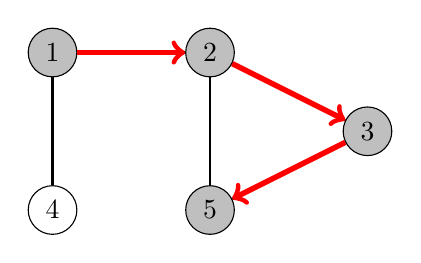
\begin{tikzpicture}
\node[draw, circle,fill=lightgray] (1) at (1,5) {$1$};
\node[draw, circle,fill=lightgray] (2) at (3,5) {$2$};
\node[draw, circle,fill=lightgray] (3) at (5,4) {$3$};
\node[draw, circle] (4) at (1,3) {$4$};
\node[draw, circle,fill=lightgray] (5) at (3,3) {$5$};

\path[draw,thick,-] (1) -- (2);
\path[draw,thick,-] (2) -- (3);
\path[draw,thick,-] (1) -- (4);
\path[draw,thick,-] (3) -- (5);
\path[draw,thick,-] (2) -- (5);

\path[draw=red,thick,->,line width=2pt] (1) -- (2);
\path[draw=red,thick,->,line width=2pt] (2) -- (3);
\path[draw=red,thick,->,line width=2pt] (3) -- (5);
\end{tikzpicture}
\end{center}
The neighbors of node 5 are 2 and 3,
but the search has already visited both of them,
so it's time to return back.
Also the neighbors of nodes 3 and 2
have been visited, so we'll next proceed
from node 1 to node 4:
\begin{center}
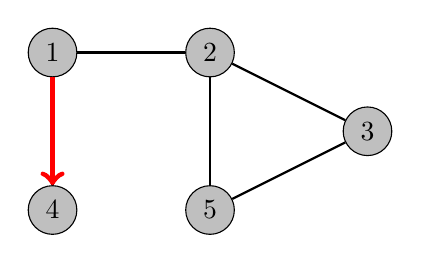
\begin{tikzpicture}
\node[draw, circle,fill=lightgray] (1) at (1,5) {$1$};
\node[draw, circle,fill=lightgray] (2) at (3,5) {$2$};
\node[draw, circle,fill=lightgray] (3) at (5,4) {$3$};
\node[draw, circle,fill=lightgray] (4) at (1,3) {$4$};
\node[draw, circle,fill=lightgray] (5) at (3,3) {$5$};

\path[draw,thick,-] (1) -- (2);
\path[draw,thick,-] (2) -- (3);
\path[draw,thick,-] (1) -- (4);
\path[draw,thick,-] (3) -- (5);
\path[draw,thick,-] (2) -- (5);

\path[draw=red,thick,->,line width=2pt] (1) -- (4);
\end{tikzpicture}
\end{center}
After this, the search terminates because it has visited
all nodes.

The time complexity of depth-first search is $O(n+m)$
where $n$ is the number of nodes and $m$ is the
number of edges,
because the algorithm processes each node and edge once.

\subsubsection*{Implementation}

Depth-first search can be conveniently
implemented using recursion.
The following function \texttt{dfs} begins
a depth-first search at a given node.
The function assumes that the graph is
stored as adjacency lists in array
\begin{lstlisting}
vector<int> v[N];
\end{lstlisting}
and also maintains an array
\begin{lstlisting}
int z[N];
\end{lstlisting}
that keeps track of the visited nodes.
Initially, each array value is 0,
and when the search arrives at node $s$,
the value of \texttt{z}[$s$] becomes 1.
The function can be implemented as follows:
\begin{lstlisting}
void dfs(int s) {
    if (z[s]) return;
    z[s] = 1;
    // process node s
    for (auto u: v[s]) {
        dfs(u);
    }
}
\end{lstlisting}

\section{Breadth-first search}

\index{breadth-first search}

\key{Breadth-first search} (BFS) visits the nodes
in increasing order of their distance
from the starting node.
Thus, we can calculate the distance
from the starting node to all other
nodes using breadth-first search.
However, breadth-first search is more difficult
to implement than depth-first search.

Breadth-first search goes through the nodes
one level after another.
First the search explores the nodes whose
distance from the starting node is 1,
then the nodes whose distance is 2, and so on.
This process continues until all nodes
have been visited.

\subsubsection*{Example}

Let's consider how the algorithm processes
the following graph:

\begin{center}
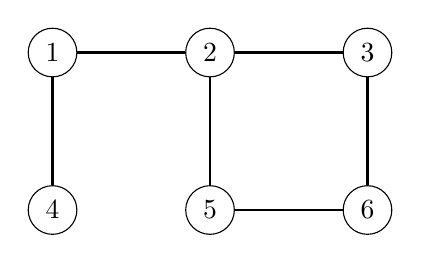
\begin{tikzpicture}
\node[draw, circle] (1) at (1,5) {$1$};
\node[draw, circle] (2) at (3,5) {$2$};
\node[draw, circle] (3) at (5,5) {$3$};
\node[draw, circle] (4) at (1,3) {$4$};
\node[draw, circle] (5) at (3,3) {$5$};
\node[draw, circle] (6) at (5,3) {$6$};


\path[draw,thick,-] (1) -- (2);
\path[draw,thick,-] (2) -- (3);
\path[draw,thick,-] (1) -- (4);
\path[draw,thick,-] (3) -- (6);
\path[draw,thick,-] (2) -- (5);
\path[draw,thick,-] (5) -- (6);
\end{tikzpicture}
\end{center}
Assume again that the search begins at node 1.
First, we process all nodes that can be reached
from node 1 using a single edge:
\begin{center}
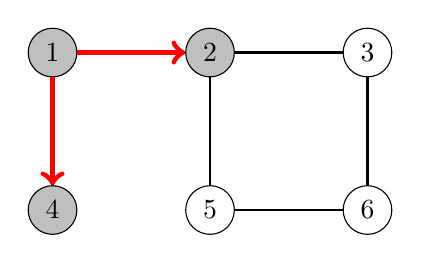
\begin{tikzpicture}
\node[draw, circle,fill=lightgray] (1) at (1,5) {$1$};
\node[draw, circle,fill=lightgray] (2) at (3,5) {$2$};
\node[draw, circle] (3) at (5,5) {$3$};
\node[draw, circle,fill=lightgray] (4) at (1,3) {$4$};
\node[draw, circle] (5) at (3,3) {$5$};
\node[draw, circle] (6) at (5,3) {$6$};

\path[draw,thick,-] (1) -- (2);
\path[draw,thick,-] (2) -- (3);
\path[draw,thick,-] (1) -- (4);
\path[draw,thick,-] (3) -- (6);
\path[draw,thick,-] (2) -- (5);
\path[draw,thick,-] (5) -- (6);

\path[draw,thick,-] (1) -- (2);
\path[draw,thick,-] (2) -- (3);
\path[draw,thick,-] (1) -- (4);
\path[draw,thick,-] (2) -- (5);

\path[draw=red,thick,->,line width=2pt] (1) -- (2);
\path[draw=red,thick,->,line width=2pt] (1) -- (4);
\end{tikzpicture}
\end{center}
After this, we procees to nodes 3 and 5:
\begin{center}
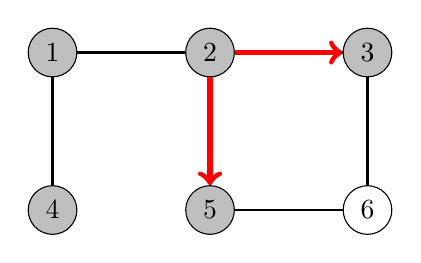
\begin{tikzpicture}
\node[draw, circle,fill=lightgray] (1) at (1,5) {$1$};
\node[draw, circle,fill=lightgray] (2) at (3,5) {$2$};
\node[draw, circle,fill=lightgray] (3) at (5,5) {$3$};
\node[draw, circle,fill=lightgray] (4) at (1,3) {$4$};
\node[draw, circle,fill=lightgray] (5) at (3,3) {$5$};
\node[draw, circle] (6) at (5,3) {$6$};

\path[draw,thick,-] (1) -- (2);
\path[draw,thick,-] (2) -- (3);
\path[draw,thick,-] (1) -- (4);
\path[draw,thick,-] (3) -- (6);
\path[draw,thick,-] (2) -- (5);
\path[draw,thick,-] (5) -- (6);

\path[draw,thick,-] (1) -- (2);
\path[draw,thick,-] (2) -- (3);
\path[draw,thick,-] (1) -- (4);
\path[draw,thick,-] (2) -- (5);

\path[draw=red,thick,->,line width=2pt] (2) -- (3);
\path[draw=red,thick,->,line width=2pt] (2) -- (5);
\end{tikzpicture}
\end{center}
Finally, we visit node 6:
\begin{center}
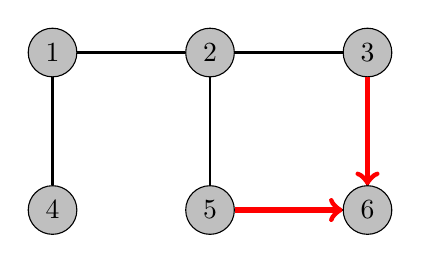
\begin{tikzpicture}
\node[draw, circle,fill=lightgray] (1) at (1,5) {$1$};
\node[draw, circle,fill=lightgray] (2) at (3,5) {$2$};
\node[draw, circle,fill=lightgray] (3) at (5,5) {$3$};
\node[draw, circle,fill=lightgray] (4) at (1,3) {$4$};
\node[draw, circle,fill=lightgray] (5) at (3,3) {$5$};
\node[draw, circle,fill=lightgray] (6) at (5,3) {$6$};

\path[draw,thick,-] (1) -- (2);
\path[draw,thick,-] (2) -- (3);
\path[draw,thick,-] (1) -- (4);
\path[draw,thick,-] (3) -- (6);
\path[draw,thick,-] (2) -- (5);
\path[draw,thick,-] (5) -- (6);

\path[draw,thick,-] (1) -- (2);
\path[draw,thick,-] (2) -- (3);
\path[draw,thick,-] (1) -- (4);
\path[draw,thick,-] (2) -- (5);

\path[draw=red,thick,->,line width=2pt] (3) -- (6);
\path[draw=red,thick,->,line width=2pt] (5) -- (6);
\end{tikzpicture}
\end{center}
Now we have calculated the distances
from the starting node to all nodes in the graph.
The distances are as follows:

\begin{tabular}{ll}
\\
node & distance \\
\hline
1 & 0 \\
2 & 1 \\
3 & 2 \\
4 & 1 \\
5 & 2 \\
6 & 3 \\
\\
\end{tabular}

Like in depth-first search,
the time complexity of breadth-first search
is $O(n+m)$ where $n$ is the number of nodes
and $m$ is the number of edges.

\subsubsection*{Implementation}

Breadth-first search is more difficult
to implement than depth-first search
because the algorithm visits nodes
in different parts in the graph.
A typical implementation is to maintain
a queue of nodes to be processed.
At each step, the next node in the queue
will be processed.

The following code begins a breadth-first
search at node $x$.
The code assumes that the graph is stored
as adjacency lists and maintains a queue
\begin{lstlisting}
queue<int> q;
\end{lstlisting}
that contains the nodes in increasing order
of their distance.
New nodes are always added to the end
of the queue, and the node at the beginning
of the queue is the next node to be processed.

In addition, the code uses arrays
\begin{lstlisting}
int z[N], e[N];
\end{lstlisting}
so that array \texttt{z} indicates
which nodes the search already has visited
and array \texttt{e} will contain the
minimum distance to all nodes in the graph.
The search can be implemented as follows:
\begin{lstlisting}
z[s] = 1; e[x] = 0;
q.push(x);
while (!q.empty()) {
    int s = q.front(); q.pop();
    // process node s
    for (auto u : v[s]) {
        if (z[u]) continue;
        z[u] = 1; e[u] = e[s]+1;
        q.push(u);
    }
}
\end{lstlisting}

\section{Sovelluksia}

Verkon läpikäynnin avulla
saa selville monia asioita
verkon rakenteesta.
Läpikäynnin voi yleensä aina toteuttaa
joko syvyyshaulla tai leveyshaulla,
mutta käytännössä syvyyshaku on parempi valinta,
koska sen toteutus on helpompi.
Oletamme seuraavaksi, että käsiteltävänä on
suuntaamaton verkko.

\subsubsection{Yhtenäisyyden tarkastaminen}

\index{yhtenxisyys@yhtenäisyys}

Verkko on yhtenäinen,
jos mistä tahansa solmuista
pääsee kaikkiin muihin solmuihin.
Niinpä verkon yhtenäisyys selviää
aloittamalla läpikäynti
jostakin verkon solmusta ja
tarkastamalla, pääseekö siitä kaikkiin solmuihin.

Esimerkiksi verkossa
\begin{center}
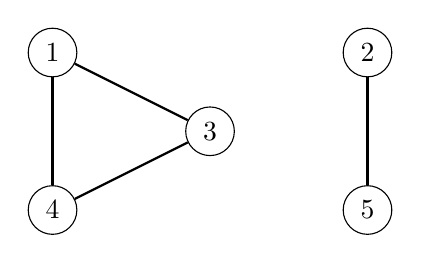
\begin{tikzpicture}
\node[draw, circle] (2) at (7,5) {$2$};
\node[draw, circle] (1) at (3,5) {$1$};
\node[draw, circle] (3) at (5,4) {$3$};
\node[draw, circle] (5) at (7,3) {$5$};
\node[draw, circle] (4) at (3,3) {$4$};

\path[draw,thick,-] (1) -- (3);
\path[draw,thick,-] (1) -- (4);
\path[draw,thick,-] (3) -- (4);
\path[draw,thick,-] (2) -- (5);
\end{tikzpicture}
\end{center}
solmusta $1$ alkava syvyyshaku löytää seuraavat
solmut:
\begin{center}
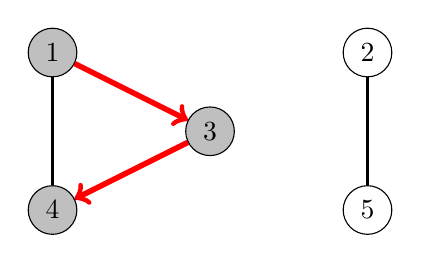
\begin{tikzpicture}
\node[draw, circle] (2) at (7,5) {$2$};
\node[draw, circle,fill=lightgray] (1) at (3,5) {$1$};
\node[draw, circle,fill=lightgray] (3) at (5,4) {$3$};
\node[draw, circle] (5) at (7,3) {$5$};
\node[draw, circle,fill=lightgray] (4) at (3,3) {$4$};

\path[draw,thick,-] (1) -- (3);
\path[draw,thick,-] (1) -- (4);
\path[draw,thick,-] (3) -- (4);
\path[draw,thick,-] (2) -- (5);

\path[draw=red,thick,->,line width=2pt] (1) -- (3);
\path[draw=red,thick,->,line width=2pt] (3) -- (4);

\end{tikzpicture}
\end{center}

Koska syvyyshaku ei pääse kaikkiin solmuihin,
tämä tarkoittaa, että verkko ei ole yhtenäinen.
Vastaavalla tavalla voi etsiä myös verkon komponentit
käymällä solmut läpi ja aloittamalla uuden syvyyshaun
aina, jos käsiteltävä solmu ei kuulu vielä mihinkään komponenttiin.

\subsubsection{Syklin etsiminen}

\index{sykli@sykli}

Verkossa on sykli,
jos jonkin komponentin läpikäynnin
aikana tulee vastaan solmu,
jonka naapuri on jo käsitelty
ja solmuun ei ole saavuttu kyseisen naapurin kautta.
Esimerkiksi verkossa
\begin{center}
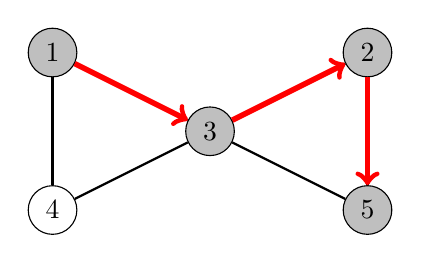
\begin{tikzpicture}
\node[draw, circle,fill=lightgray] (2) at (7,5) {$2$};
\node[draw, circle,fill=lightgray] (1) at (3,5) {$1$};
\node[draw, circle,fill=lightgray] (3) at (5,4) {$3$};
\node[draw, circle,fill=lightgray] (5) at (7,3) {$5$};
\node[draw, circle] (4) at (3,3) {$4$};

\path[draw,thick,-] (1) -- (3);
\path[draw,thick,-] (1) -- (4);
\path[draw,thick,-] (3) -- (4);
\path[draw,thick,-] (2) -- (5);
\path[draw,thick,-] (2) -- (3);
\path[draw,thick,-] (3) -- (5);

\path[draw=red,thick,->,line width=2pt] (1) -- (3);
\path[draw=red,thick,->,line width=2pt] (3) -- (2);
\path[draw=red,thick,->,line width=2pt] (2) -- (5);

\end{tikzpicture}
\end{center}
on sykli, koska tultaessa solmusta 2 solmuun 5
havaitaan, että naapurina oleva solmu 3 on jo käsitelty.
Niinpä verkossa täytyy olla solmun 3 kautta
kulkeva sykli.
Tällainen sykli on esimerkiksi
$3 \rightarrow 2 \rightarrow 5 \rightarrow 3$.

Syklin olemassaolon voi myös päätellä laskemalla,
montako solmua ja kaarta komponentissa on.
Jos komponentissa on $c$ solmua ja siinä ei ole sykliä,
niin siinä on oltava tarkalleen $c-1$ kaarta.
Jos kaaria on $c$ tai enemmän, niin komponentissa
on varmasti sykli.

\subsubsection{Kaksijakoisuuden tarkastaminen}

\index{kaksijakoisuus@kaksijakoisuus}

Verkko on kaksijakoinen,
jos sen solmut voi värittää
kahdella värillä
niin, että kahta samanväristä
solmua ei ole vierekkäin.
On yllättävän helppoa selvittää
verkon läpikäynnin avulla,
onko verkko kaksijakoinen.

Ideana on värittää alkusolmu
siniseksi, sen kaikki naapurit
punaiseksi, niiden kaikki naapurit
siniseksi, jne.
Jos jossain vaiheessa
ilmenee ristiriita
(saman solmun tulisi olla sekä
sininen että punainen),
verkko ei ole kaksijakoinen.
Muuten verkko on kaksijakoinen
ja yksi väritys on muodostunut.

Esimerkiksi verkko
\begin{center}
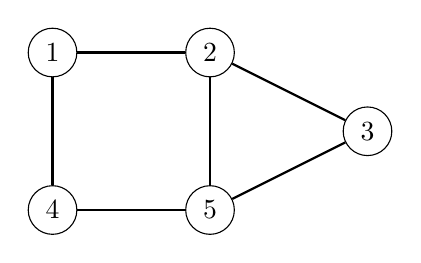
\begin{tikzpicture}
\node[draw, circle] (2) at (5,5) {$2$};
\node[draw, circle] (1) at (3,5) {$1$};
\node[draw, circle] (3) at (7,4) {$3$};
\node[draw, circle] (5) at (5,3) {$5$};
\node[draw, circle] (4) at (3,3) {$4$};

\path[draw,thick,-] (1) -- (2);
\path[draw,thick,-] (2) -- (5);
\path[draw,thick,-] (5) -- (4);
\path[draw,thick,-] (4) -- (1);
\path[draw,thick,-] (2) -- (3);
\path[draw,thick,-] (5) -- (3);
\end{tikzpicture}
\end{center}
ei ole kaksijakoinen, koska
läpikäynti solmusta 1 alkaen
aiheuttaa seuraavan ristiriidan:
\begin{center}
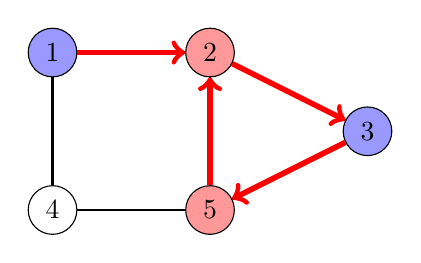
\begin{tikzpicture}
\node[draw, circle,fill=red!40] (2) at (5,5) {$2$};
\node[draw, circle,fill=blue!40] (1) at (3,5) {$1$};
\node[draw, circle,fill=blue!40] (3) at (7,4) {$3$};
\node[draw, circle,fill=red!40] (5) at (5,3) {$5$};
\node[draw, circle] (4) at (3,3) {$4$};

\path[draw,thick,-] (1) -- (2);
\path[draw,thick,-] (2) -- (5);
\path[draw,thick,-] (5) -- (4);
\path[draw,thick,-] (4) -- (1);
\path[draw,thick,-] (2) -- (3);
\path[draw,thick,-] (5) -- (3);

\path[draw=red,thick,->,line width=2pt] (1) -- (2);
\path[draw=red,thick,->,line width=2pt] (2) -- (3);
\path[draw=red,thick,->,line width=2pt] (3) -- (5);
\path[draw=red,thick,->,line width=2pt] (5) -- (2);
\end{tikzpicture}
\end{center}
Tässä vaiheessa havaitaan,
että sekä solmun 2 että solmun 5 väri on punainen,
vaikka solmut ovat vierekkäin verkossa,
joten verkko ei ole kaksijakoinen.

Tämä algoritmi on luotettava tapa selvittää
verkon kaksijakoisuus,
koska kun värejä on vain kaksi,
ensimmäisen solmun värin valinta
määrittää kaikkien muiden
samassa komponentissa olevien
solmujen värin.
Ei ole merkitystä,
kumman värin ensimmäinen
solmu saa.

Huomaa, että yleensä ottaen on vaikeaa
selvittää, voiko verkon solmut
värittää $k$ värillä niin,
ettei missään kohtaa ole vierekkäin
kahta samanväristä solmua.
Edes tapaukseen $k=3$ ei tunneta
mitään tehokasta algoritmia,
vaan kyseessä on NP-vaikea ongelma.
% 
% \section{Labyrintin käsittely}
% 
% Labyrintti on ruudukko, joka muodostuu lattia- ja seinäruuduista,
% ja labyrintissa on sallittua kulkea lattiaruutuja pitkin.
% Labyrinttia
% \begin{center}
% \begin{tikzpicture}[scale=0.7]
% \fill[color=gray] (0,0) rectangle (8,1);
% \fill[color=gray] (0,5) rectangle (8,6);
% \fill[color=gray] (0,0) rectangle (1,6);
% \fill[color=gray] (7,0) rectangle (8,6);
% 
% \fill[color=gray] (2,0) rectangle (3,4);
% \fill[color=gray] (4,2) rectangle (6,4);
% 
% \draw (0,0) grid (8,6);
% 
% \node at (1.5,1.5) {$a$};
% \node at (6.5,3.5) {$b$};
% \end{tikzpicture}
% \end{center}
% vastaa luontevasti verkko
% \begin{center}
% \begin{tikzpicture}[scale=0.7]
% \node[draw,circle,minimum size=20pt] (a) at (1,1) {$a$};
% \node[draw,circle,minimum size=20pt] (b) at (1,2.5) {};
% \node[draw,circle,minimum size=20pt] (c) at (1,4) {};
% \node[draw,circle,minimum size=20pt] (d) at (1,5.5) {};
% \node[draw,circle,minimum size=20pt] (e) at (2.5,5.5) {};
% \node[draw,circle,minimum size=20pt] (f) at (4,5.5) {};
% \node[draw,circle,minimum size=20pt] (g) at (5.5,5.5) {};
% \node[draw,circle,minimum size=20pt] (h) at (7,5.5) {};
% \node[draw,circle,minimum size=20pt] (i) at (8.5,5.5) {};
% \node[draw,circle,minimum size=20pt] (j) at (8.5,4) {$b$};
% \node[draw,circle,minimum size=20pt] (k) at (8.5,2.5) {};
% \node[draw,circle,minimum size=20pt] (l) at (8.5,1) {};
% \node[draw,circle,minimum size=20pt] (m) at (7,1) {};
% \node[draw,circle,minimum size=20pt] (n) at (5.5,1) {};
% \node[draw,circle,minimum size=20pt] (o) at (4,1) {};
% \node[draw,circle,minimum size=20pt] (p) at (4,2.5) {};
% \node[draw,circle,minimum size=20pt] (q) at (4,4) {};
% 
% \path[draw,thick,-] (a) -- (b);
% \path[draw,thick,-] (b) -- (c);
% \path[draw,thick,-] (c) -- (d);
% \path[draw,thick,-] (d) -- (e);
% \path[draw,thick,-] (e) -- (f);
% \path[draw,thick,-] (f) -- (g);
% \path[draw,thick,-] (g) -- (h);
% \path[draw,thick,-] (h) -- (i);
% \path[draw,thick,-] (i) -- (j);
% \path[draw,thick,-] (j) -- (k);
% \path[draw,thick,-] (k) -- (l);
% \path[draw,thick,-] (l) -- (m);
% \path[draw,thick,-] (m) -- (n);
% \path[draw,thick,-] (n) -- (o);
% \path[draw,thick,-] (o) -- (p);
% \path[draw,thick,-] (p) -- (q);
% \path[draw,thick,-] (q) -- (f);
% \end{tikzpicture}
% \end{center}
% jossa verkon solmuja ovat labyrintin lattiaruudut
% ja solmujen välillä on kaari, jos lattiaruudusta
% toiseen pääsee kulkemaan yhdellä askeleella.
% Niinpä erilaiset labyrinttiin liittyvät ongelmat
% palautuvat verkko-ongelmiksi.
% 
% Esimerkiksi syvyyshaulla pystyy selvittämään,
% onko ruudusta $a$ reittiä ruutuun $b$
% ja leveyshaku kertoo lisäksi,
% mikä on pienin mahdollinen askelten määrä reitillä.
% Samoin voi esimerkiksi vaikkapa, kuinka monta
% toisistaan erillistä huonetta labyrintissa on
% sekä kuinka monta ruutua huoneissa on.
% 
% Labyrintin tapauksessa ei kannata muodostaa erikseen
% verkkoa, vaan syvyyshaun ja leveyshaun voi toteuttaa
% suoraan labyrintin ruudukkoon.

